\section{Auswertung}
\label{sec:Auswertung}

\subsection{Flächenträgheitsmoment und Dichte}

  Zur Bestimmung des Flächenträgheitsmoments und der Dichte des Stabes werden für Masse, Durchmesser und Länge mehrere
  Werte von jeweils einem runden und einem eckigen Stab notiert. Diese lassen sich in \autoref{tab:runder_Stab} und \autoref{tab:eckiger_Stab} finden.

  \begin{table}
    \centering
    \caption{Messdaten des runden Stabes}
    \label{tab:runder_Stab}
    \begin{tabular}{c c c}
      \toprule
      Masse/kg & Radius/m & Länge/m \\
      \midrule
      0,4120 & 0,005 & 0,592 \\
      0,4119 & 0,005 & 0,593 \\
      0,4120 & 0,005 & 0,592 \\
      0,4124 & 0,005 & 0,593 \\
      0,4123 & 0,005 & 0,591 \\
      \bottomrule
    \end{tabular}
  \end{table}

  Die folgenden Mittelwerte und Standardabweichungen der Werte werden mittels Python bestimmt.\\
  Masse des runden Stabs: $m_{\symup{\bigcirc}} = 0{,}41212 \pm 0{,}00019 \, \mathrm{kg}$\\
  Radius des runden Stabs: $r_{\symup{\bigcirc}} = 0{,}0050 \pm 0 \, \mathrm{m}$\\
  Länge des runden Stabs: $l_{\symup{\bigcirc}} = 0{,}5922 \pm 0{,}0007 \, \mathrm{m}$\\

  \begin{table}
    \centering
    \caption{Messdaten des eckigen Stabes}
    \label{tab:eckiger_Stab}
    \begin{tabular}{c c c}
      \toprule
      Masse/kg & Durchmesser/m & Länge/m \\
      \midrule
      0,5357 & 0,01 & 0,602 \\
      0,5359 & 0,01 & 0,601 \\
      0,5360 & 0,01 & 0,602 \\
      0,5360 & 0,01 & 0,601 \\
      0,5360 & 0,01 & 0,602 \\
      \bottomrule
    \end{tabular}
  \end{table}
  Masse des eckigen Stabs: $m_{\symup{\square}} = 0{,}53592 \pm 0{,}00012 \, \mathrm{kg}$\\
  Durchmesser des eckigen Stabs: $r_{\symup{\square}} = 0{,}0100 \pm 0 \, \mathrm{m}$\\
  Länge des eckigen Stabs: $l_{\symup{\square}} = 0{,}6016 \pm 0{,}0005 \, \mathrm{m}$\\
  \\
  \subsubsection{Dichte}
    Die Dichte eines Zylinders bestimmt sich zu: $\rho_{\symup{\bigcirc}} = \frac{m}{r^2 \, \pi \, l}$.\\
    Somit ergibt sich mit den Messwerten die Dichte des Zylinders zu $\rho_{\symup{\bigcirc}} = 8860 \pm 11 \, \frac{\mathrm{kg}}{\mathrm{m^3}}$.\\

    Die Dichte eines Quader bestimmt sich zu: $\rho_{\symup{\square}} = \frac{m}{d^2 \, l}$.\\
    Somit ergibt sich mit den Messwerten die Dichte des Quaders zu $\rho_{\symup{\square}} = 8908 \pm 8 \, \frac{\mathrm{kg}}{\mathrm{m^3}}$.\\

    Der Dichte nach zu urteilen, könnte es sich bei dem Material der Stäbe um Kupfer handeln, was sich durch das visuelle
    Erscheinungsbild bestätigen lässt. Somit haben die Stäbe einen Literaturwert für den Elastizitätsmodul von $E_{\mathrm{lit}} = 100 \text{ bis } 130 \cdot \mathrm{10^{9}} \frac{\mathrm{N}}{m^2}$\cite{Kupfer}.
  \subsubsection{Flächenträgheitsmoment}

  Mit der \autoref{eqn:quadrat} ergibt sich für den eckigen Stab das Flächenträgheitsmoment $I_{\symup{\square}} = 8,333 \cdot 10^{-10} \, \mathrm{m^4}$ und mit \autoref{eqn:kreis} für den 
  runden Stab das Flächenträgheitsmoment $I_{\symup{\bigcirc}} = 4,909 \cdot 10^{-10} \, \mathrm{m^4}$.\\

\subsection{Bestimmung des Elastizitätsmoduls mithilfe einseitiger Einspannung}

\subsubsection{Runder Stab}
  Der Stab wird für diesen Versuch einseitig eingespannt und die restliche Länge des Stabes sechs Mal gemessen und gemittelt:

  \begin{table}
    \centering
    \caption{Restliche Länge des Stabes nach Einspannen}
    \label{tab:einseitig_runder_Laenge}
    \begin{tabular}{c}
      \toprule
      Länge/m \\
      \midrule
      0,481 \\
      0,480 \\
      0,479 \\
      0,480 \\
      0,478 \\
      0,480 \\
      \bottomrule
    \end{tabular}
  \end{table}

  Somit ergibt sich für die Länge $L = 0{,}4797 \pm 0,0009 \, \mathrm{m}$.\\

  Für die Messung wurde ein Gewicht verwendet, das mehrfach gewogen wird. Die Messwerte befinden sich in \autoref{tab:Gewicht1}.

  \begin{table}
    \centering
    \caption{Verwendetes Gewicht für die einseitige Spannung des runden Stabs}
    \label{tab:Gewicht1}
    \begin{tabular}{c}
      \toprule
      Gewicht/kg \\
      \midrule
      0,4511 \\
      0,4515 \\
      0,4515 \\
      0,4511 \\
      0,4513 \\
      \bottomrule
    \end{tabular}
  \end{table}

  Somit ergibt sich für das Gewicht die Masse $m = 0{,}4513 \pm 0,0002 \, \mathrm{kg}$.\\

  Es wird zunächst eine Messung ohne Gewicht durchgeführt, um mögliche Verbiegungen des Stabes zu erkennen. Danach wird eine Messung mit
  dem Gewicht durchgeführt. Daraus wird dann die tatsächliche Auslenkung bestimmt. In den folgenden Versuchen wird das gleiche Schema verwendet. Die Werte zu der ersten
  Messreihe lassen sich in \autoref{tab:einseitig_runder_Nullauslenkung} finden.

  \begin{table}
    \centering
    \caption{Auslenkung des runden Stabes bei einseitiger Einspannung}
    \label{tab:einseitig_runder_Nullauslenkung}
    \begin{tabular}{c c c c}
      \toprule
      $x$/mm & $\mathrm{D_0(x)}/\mathrm{mm}$ & $\mathrm{D_m(x)}/\mathrm{mm}$ & $\mathrm{D(x)}/\mathrm{mm}$ \\
      \midrule
      30 & 0,040 & 0,050 & 0,010 \\
      60 & 0,050 & 0,150 & 0,100 \\
      90 & 0,150 & 0,350 & 0,200 \\
      120 & 0,295 & 0,630 & 0,335 \\
      150 & 0,520 & 0,990 & 0,470 \\
      180 & 0,740 & 1,410 & 0,670 \\
      210 & 0,960 & 1,830 & 0,870 \\
      240 & 1,260 & 2,245 & 0,985 \\
      270 & 1,530 & 2,750 & 1,220 \\
      300 & 1,825 & 3,290 & 1,465 \\
      330 & 2,190 & 3,850 & 1,660 \\
      360 & 2,505 & 4,180 & 1,675 \\
      390 & 2,880 & 4,760 & 1,880 \\
      420 & 3,360 & 5,370 & 2,010 \\
      450 & 3,710 & 6,160 & 2,450 \\
      \bottomrule
    \end{tabular}
  \end{table}

  Hierbei ist $x$ die Entfernung zur Einspannung, $D_0(x)$ die Auslenkung des Stabes ohne Gewicht, $D_m(x)$ die Auslenkung des Stabes mit Gewicht und
  $D(x)$ die tatsächliche Auslenkung. Ein negativer Wert für $D_0$ steht für eine Auslenkung nach oben und ein positiver Wert für eine Auslenkung nach unten.\\

  Zur Berechnung des Elastizitätsmoduls E wird $D(x)$ nun gegen $\left(Lx^2-\frac{x^3}{3}\right)$ aufgetragen und eine Ausgleichsrechnung mittels Python durchgeführt. Dieser
  Zusammenhang lässt sich in \autoref{eqn:Durchbiegung} ablesen.\\
  Die Ausgleichsrechnung ergibt für diese Messreihe einen Wert für den Elastizitätsmodul von $E_1 = (120{,}3 \pm 3{,}285) \cdot \mathrm{10^{9}} \frac{\mathrm{N}}{m^2}$. Der passende Plot dazu ist
  \autoref{fig:Messwerte1}.

  \begin{figure}
    \centering
    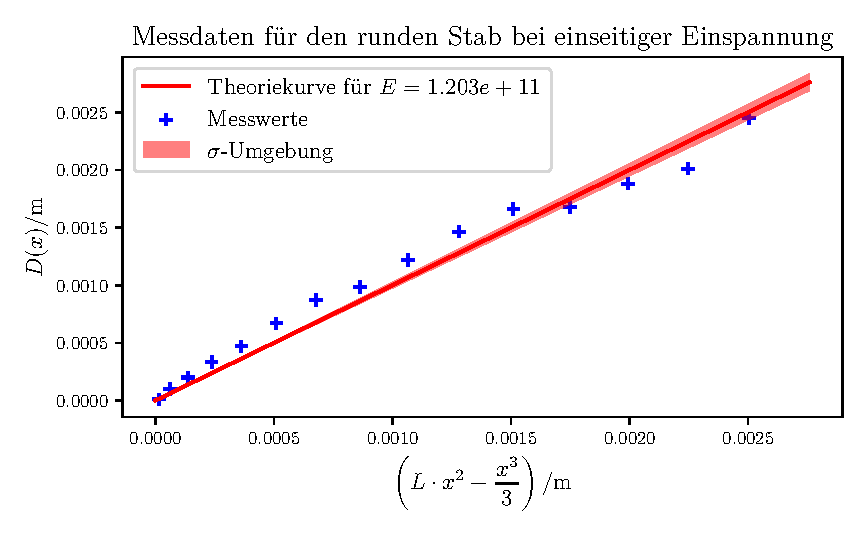
\includegraphics{build/plot2.pdf}
    \caption{Ausgleichsrechnung für das E-Modul des runden Stabs bei einseitiger Einspannung}
    \label{fig:Messwerte1}
  \end{figure}

  \newpage

\subsubsection{Eckiger Stab}
  Der Stab wird wie auch der Runde einseitig eingespannt und die restliche Länge des Stabes fünf Mal gemessen und gemittelt:

  \begin{table}
    \centering
    \caption{Restliche Länge des Stabes nach Einspannen}
    \label{tab:einseitig_eckiger_Laenge}
    \begin{tabular}{c}
      \toprule
      Länge/m \\
      \midrule
      0,488 \\
      0,489 \\
      0,488 \\
      0,489 \\
      0,487 \\
      \bottomrule
    \end{tabular}
  \end{table}

  Somit ergibt sich für Die Länge $L = 0{,}4882 \pm 0,0007 \, \mathrm{m}$.\\

  Für die Messung wird wieder ein Gewicht verwendet, das mehrfach gewogen wird. Die Messwerte finden sich in \autoref{tab:Gewicht2}.

  \begin{table}
    \centering
    \caption{Verwendetes Gewicht für die einseitige Spannung des eckigen Stabs}
    \label{tab:Gewicht2}
    \begin{tabular}{c}
      \toprule
      Gewicht/kg \\
      \midrule
      0,6529 \\
      0,6529 \\
      0,6529 \\
      0,6528 \\
      0,6528 \\
      \bottomrule
    \end{tabular}
  \end{table}

  Somit ergibt sich für das Gewicht die Masse $m = 0{,}6529 \pm 0,0000 \, \mathrm{kg}$.\\

  Es wird wie bei dem runden Stab vorgegangen. Die Werte dazu lassen
  sich in \autoref{tab:einseitig_eckiger_Nullauslenkung} finden.

  \begin{table}
    \centering
    \caption{Auslenkung des eckigen Stabes bei einseitiger Einspannung}
    \label{tab:einseitig_eckiger_Nullauslenkung}
    \begin{tabular}{c c c c}
      \toprule
      $x$/mm & $\mathrm{D_0(x)}/\mathrm{mm}$ & $\mathrm{D_m(x)}/\mathrm{mm}$ & $\mathrm{D(x)}/\mathrm{mm}$ \\
      \midrule
      30 & 0,300 & 0,330 & 0,030 \\
      60 & 0,340 & 0,420 & 0,080 \\
      90 & 0,400 & 0,550 & 0,150 \\
      120 & 0,470 & 0,750 & 0,280 \\
      150 & 0,610 & 1,000 & 0,390 \\
      180 & 0,780 & 1,340 & 0,560 \\
      210 & 0,850 & 1,550 & 0,700 \\
      240 & 0,970 & 1,840 & 0,870 \\
      270 & 1,080 & 2,130 & 1,050 \\
      300 & 1,190 & 2,470 & 1,280 \\
      330 & 1,310 & 2,780 & 1,470 \\
      360 & 1,420 & 3,120 & 1,700 \\
      390 & 1,620 & 3,530 & 1,910 \\
      420 & 1,840 & 4,000 & 2,160 \\
      450 & 2,270 & 4,430 & 2,160 \\
      \bottomrule
    \end{tabular}
  \end{table}

  Für die Messreihe mit dem eckigen Stab ergibt dies einen Wert für den Elastizitätsmodul von $E_2 = (110{,}8 \pm 1{,}753) \cdot \mathrm{10^{9}} \frac{\mathrm{N}}{m^2}$. Der passende Plot dazu ist
  \autoref{fig:Messwerte2}.

  \begin{figure}
    \centering
    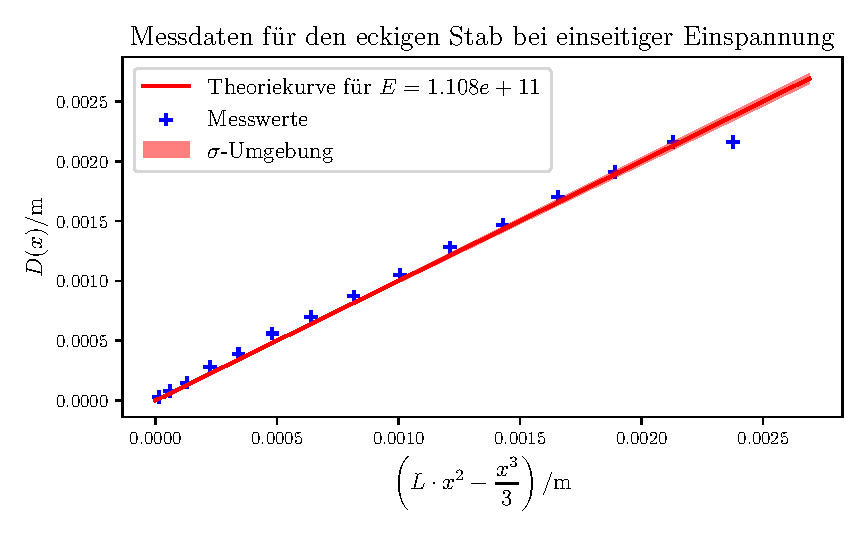
\includegraphics{build/plot3.pdf}
    \caption{Ausgleichsrechnung für das E-Modul des eckigen Stabs bei einseitiger Einspannung}
    \label{fig:Messwerte2}
  \end{figure}
  \newpage

\subsection{Bestimmung des Elastizitätsmoduls mithilfe beidseitiger Auflage}

\subsubsection{Runder Stab}
  Der Stab wird für diesen Versuch beidseitig aufgelegt und die Länge zwischen den Auflagepunten fünf Mal gemessen und gemittelt:

  \begin{table}
    \centering
    \caption{Länge des runden Stabes zwischen den Auflagepunkte}
    \label{tab:beidseitig_runder_Laenge}
    \begin{tabular}{c}
      \toprule
      Länge/m \\
      \midrule
      0,554 \\
      0,553 \\
      0,553 \\
      0,554 \\
      0,553 \\
      \bottomrule
    \end{tabular}
  \end{table}

  Somit ergibt sich für die Länge $L = 0{,}5534 \pm 0,0005 \, \mathrm{m}$.\\

  Für die Messung wird ein Gewicht verwendet, das mehrfach gewogen wird. Die Messwerte finden sich in \autoref{tab:Gewicht3}.

  \begin{table}
    \centering
    \caption{Verwendetes Gewicht für die beidseitige Auflage des runden Stabs}
    \label{tab:Gewicht3}
    \begin{tabular}{c}
      \toprule
      Gewicht/kg \\
      \midrule
      1,4535 \\
      1,4534 \\
      1,4534 \\
      1,4534 \\
      1,4533 \\
      \bottomrule
    \end{tabular}
  \end{table}

  Somit ergibt sich für das Gewicht die Masse $m = 1{,}4534 \pm 0,0001 \, \mathrm{kg}$.\\

  Es wird wie bei den anderen Versuchen vorgegangen. Die Werte dazu lassen
  sich in \autoref{tab:beidseitig_runder_Nullauslenkung} finden.

  \begin{table}
    \centering
    \caption{Auslenkung des runden Stabes bei beidseitiger Auflage}
    \label{tab:beidseitig_runder_Nullauslenkung}
    \begin{tabular}{c c c c}
      \toprule
      $x$/mm & $\mathrm{D_0(x)}/\mathrm{mm}$ & $\mathrm{D_m(x)}/\mathrm{mm}$ & $\mathrm{D(x)}/\mathrm{mm}$ \\
      \midrule
      30 & -0,250 & -0,090 & 0,160 \\
      60 & -0,340 & -0,070 & 0,270 \\
      90 & -0,380 & 0,000 & 0,380 \\
      120 & -0,360 & 0,120 & 0,480\\
      150 & -0,290 & 0,265 & 0,555 \\
      180 & -0,270 & 0,410 & 0,680 \\
      210 & -0,280 & 0,490 & 0,770 \\
      240 & -0,210 & 0,510 & 0,720 \\
      270 & -0,140 & 0,520 & 0,660 \\
      300 & -0,060 & 0,540 & 0,600\\
      330 & 0,040 & 0,550 & 0,510\\
      360 & 0,080 & 0,550 & 0,470\\
      390 & 0,170 & 0,560 & 0,390\\
      420 & 0,250 & 0,560 & 0,310 \\
      450 & 0,320 & 0,520 & 0,200\\
      480 & 0,400 & 0,520 & 0,120\\
      510 & 0,420 & 0,470 & 0,050\\
      540 & 0,330 & 0,380 & 0,050\\
      \bottomrule
    \end{tabular}
  \end{table}

  Hierbei ist $x$ die Entfernung zu der rechten aufgelegten Seite des Stabes, $D_0(x)$ die Auslenkung des Stabes ohne Gewicht, $D_m(x)$ die Auslenkung des Stabes mit Gewicht und
  $D(x)$ die tatsächliche Auslenkung. Ein negativer Wert für $D_0$ steht für eine Auslenkung nach oben und ein positiver Wert für eine Auslenkung nach unten. Das Gewicht wurde diesmal
  nicht am Ende des Stabes, sondern mittig bei $x=27,5 \, \mathrm{cm}$ aufgehangen.\\

  Zur Berechnung des Elastizitätsmoduls E wird $D(x)$ nun gegen $\left(3L^2x -4x^3\right)$ und $\left(4x^3 -12Lx^2 +9L^2 x - L^3\right)$ aufgetragen und eine Ausgleichsrechnung mittels Python durchgeführt. 
  Der Zusammenhang lässt sich an \autoref{eqn:DurchbiegungL/2} und \autoref{eqn:DurchbiegungL} ablesen. Im Bereich von $0 \leq x \leq L/2$ wird \autoref{eqn:DurchbiegungL/2} verwendet und im Bereich $L/2 \leq x \leq L$ 
  \autoref{eqn:DurchbiegungL}.\\
  Das ergibt für diese Messreihe einen Wert für der Elastizitätsmodul von $E_3 = (156{,}6 \pm 8{,}339) \cdot \mathrm{10^{9}} \frac{\mathrm{N}}{m^2}$. Der passende Plot dazu ist
  \autoref{fig:Messwerte3}.

  \begin{figure}
    \centering
    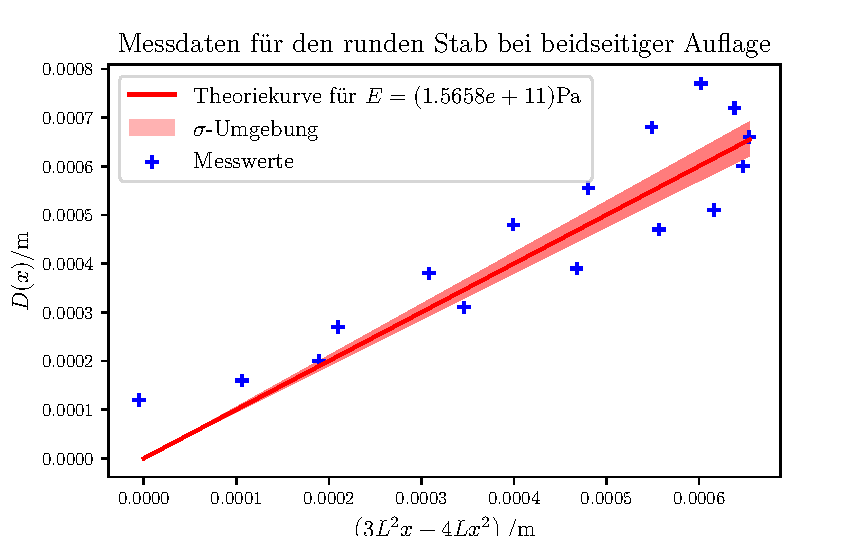
\includegraphics{build/plot4.pdf}
    \caption{Ausgleichsrechnung für das E-Modul des runden Stabs bei beidseitiger Auflage}
    \label{fig:Messwerte3}
  \end{figure}
  \newpage

\subsubsection{Eckiger Stab}
  Der Stab wird für diesen Versuch beidseitig aufgelegt und die Länge zwischen den Auflagepunkten fünf Mal gemessen und gemittelt:

  \begin{table}
    \centering
    \caption{Länge des eckigen Stabes zwischen den Auflagepunkten}
    \label{tab:beidseitig_eckiger_Laenge}
    \begin{tabular}{c}
      \toprule
      Länge/m \\
      \midrule
      0,557 \\
      0,558 \\
      0,556 \\
      0,557 \\
      0,558 \\
      \bottomrule
    \end{tabular}
  \end{table}

  Somit ergibt sich für die Länge $L = 0{,}5572 \pm 0,0007 \, \mathrm{m}$.\\

  Für die Messung wird ein Gewicht verwendet, das mehrfach gewogen wird. Die Messwerte finden sich in \autoref{tab:Gewicht4}.

  \begin{table}
    \centering
    \caption{Verwendetes Gewicht für die beidseitige Auflage des eckigen Stabs}
    \label{tab:Gewicht4}
    \begin{tabular}{c}
      \toprule
      Gewicht/kg \\
      \midrule
      1.5522\\
      1.5529 \\
      1.5528 \\
      1.5530 \\
      1.5530  \\
      \bottomrule
    \end{tabular}
  \end{table}

  Somit ergibt sich für das Gewicht die Masse $m = 1{,}5528 \pm 0,0003 \, \mathrm{kg}$.\\

  Vorgehen und Bezeichnungen sind identisch zu dem Versuch mit dem runden Stab. Die Werte dazu lassen
  sich in \autoref{tab:beidseitig_eckiger_Nullauslenkung} finden.\\

  \begin{table}
    \centering
    \caption{Auslenkung des eckigen Stabes bei beidseitiger Auflage}
    \label{tab:beidseitig_eckiger_Nullauslenkung}
    \begin{tabular}{c c c c}
      \toprule
      $x$/mm & $\mathrm{D_0(x)}/\mathrm{mm}$ & $\mathrm{D_m(x)}/\mathrm{mm}$ & $\mathrm{D(x)}/\mathrm{mm}$ \\
      \midrule
      30 & -0.050 & 0.190 & 0.240 \\
      60 & -0.140 & 0.200 & 0.340 \\
      90 & -0.210 & 0.210 & 0.420\\
      120 & -0.270 & 0.230 & 0.500\\
      150 & -0.350 & 0.210 & 0.560 \\
      180 & -0.400 & 0.220 & 0.620 \\
      210 & -0.510 & 0.150 & 0.660 \\
      240 & -0.540 & 0.120 & 0.660 \\
      270 & -0.620 & 0.070 & 0.690 \\
      300 & -0.740 & -0.260 & 0.480\\
      330 & -0.860 & -0.420 & 0.440\\
      360 & -1.000 & -0.600 & 0.400\\
      390 & -1.110 & -0.800 & 0.310\\
      420 & -1.250 & -1.000 & 0.250 \\
      450 & -1.350 & -1.220 & 0.130\\
      480 & -1.420 & -1.310 & 0.110\\
      510 & -1.660 & -1.570 & 0.090\\
      540 & -1.770 & -1.760 & 0.010\\
      \bottomrule
    \end{tabular}
  \end{table}

  Zur Berechnung des Elastizitätsmoduls E wird $D(x)$ nun wieder gegen $\left(3L^2x -4x^3\right)$ und $\left(4x^3 -12Lx^2 +9L^2 x - L^3\right)$ aufgetragen und eine Ausgleichsrechnung mittels Python durchgeführt.\\
  Das ergibt für diese Messreihe einen Wert für des Elastizitätsmoduls von $E_4 = (100{,}2 \pm 5{,}333) \cdot \mathrm{10^{9}} \frac{\mathrm{N}}{m^2}$. Der passende Plot dazu ist
  \autoref{fig:Messwerte4}.

  \begin{figure}
    \centering
    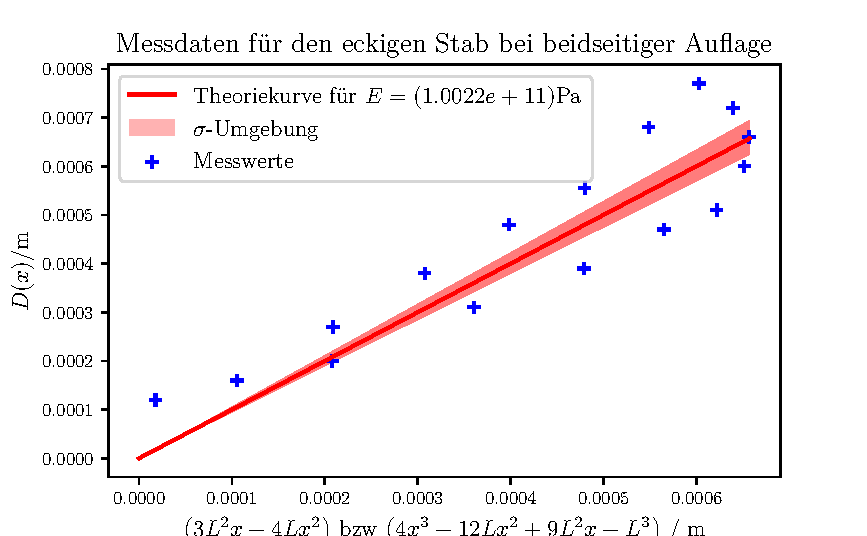
\includegraphics{build/plot9.pdf}
    \caption{Ausgleichsrechnung für das E-Modul des eckigen Stabs bei beidseitiger Auflage}
    \label{fig:Messwerte4}
  \end{figure}
  \newpage
